\chapter{Cross-lingual Word Sense Disambiguation}
\label{sec:clwsd}

Cross-lingual word sense disambiguation (CL-WSD) is the task of labeling words
or phrases in some input text with their contextually-appropriate translations
into some target language.
It is a variant of the more general WSD task, with the sense inventory for each
word defined as its possible translations.
This setting for WSD has immediate applications in both machine translation and
cross-language information retrieval, since many words have multiple possible
translations.

WSD in translation has a long history; practical work in integrating
WSD with statistical machine translation dates back to early SMT work at IBM
\cite{Brown91word-sensedisambiguation}, but the problem itself was described in
Warren Weaver's prescient 1949 memorandum \cite{weavermemo}, which describes an
essentially modern conception of word sense disambiguation.

In the early history of machine translation, researchers were very concerned
with WSD; to some, it seemed an insurmountable problem. Bar-Hillel 
discussed the difficulty of writing a program to translate sentences with
simple ambiguities like \emph{The box was in the pen.} \cite{barhillel1960}:

\begin{quote}
... I know of no program that would enable a machine to come up with this
unique rendering unless by a completely arbitrary and ad hoc procedure whose
futility would show itself ...
\end{quote}

To produce a correct rendering of this sentence in Spanish, for example, the
translation system must decide between translating ``pen" as \emph{corral} (an
enclosure, like for an animal) or as \emph{pluma} (the instrument for writing).
As of this writing, for this particular example, Google Translate picks the
less-sensible ``in the writing implement" translation (see Figure
\ref{fig:box-in-pen}).
One wonders how this could come about -- we would hope that the n-gram language
model for Spanish would prefer sentences about things in enclosures to things
in writing implements.
But the word \emph{en} can be a translation of either the English ``in" or
``on", and \emph{pluma} can also mean ``feather".
The situation is fairly complex.


\begin{figure}
  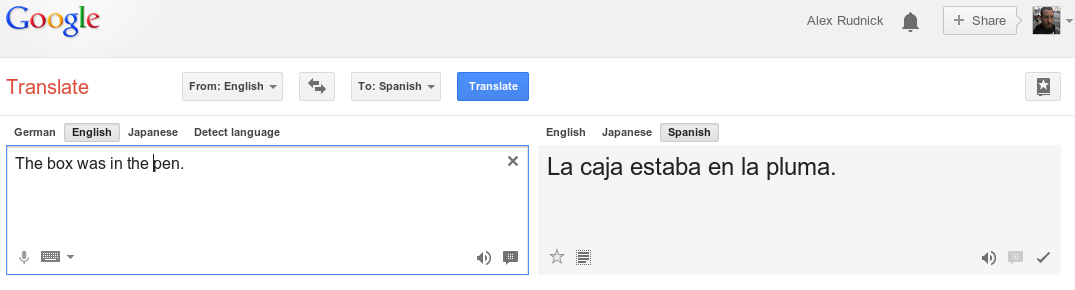
\includegraphics[width=12cm]{box-in-pen.png}
  \caption{Google Translate, September 17, 2013; interestingly, adding or
  removing the final period in the English sentence causes a switch between the
  ``pluma" and ``corral" renderings.}
  \label{fig:box-in-pen}
\end{figure}

In general, there is a many-to-many relationship between words across language
boundaries.
This happens for a number of reasons: figurative or metaphorical uses may not
translate directly,
obligatory information in one language may be left unspecified in another,
or the criteria for selecting a word may simply differ.
To give some familiar examples, a ``leg" of a trip in English is typically
translated as \emph{etape} in French, which is unrelated to limbs used for
walking;
translating ``brother" to Japanese requires specifying whether the brother is
older (\emph{ani}) or younger (\emph{ot\=oto});
a soap bubble or a ceramic plate can be destroyed with the same word in
Chinese, whereas English speakers typically distinguish between the verbs
``pop" and ``break" \cite{majid2007semantic}.

Despite these difficulties, most statistical MT systems do not use an explicit
WSD module \cite{wsdchap3}; the language model and phrase tables of these
systems mitigate lexical ambiguities by encouraging words used collocationally
to appear together in the output. Entire phrases\footnote{Not necessarily
``phrases" in a syntactic sense, but subsequences of sentences} such as verbs
with their common objects may be learned and stored in the phrase table, and
the language model will encourage common collocations as well.

To take a look at some apparently easier examples, let us also consider the
following usages of \emph{letter}, from the test set of a recent SemEval shared
task \cite{task10}, and how to translate them into Spanish.

\enumsentence{
But a quick look at today's \emph{letters} to the editor in the Times suggest
that here at least is one department of the paper that could use a little more
fact-checking. }
\label{sent:carta}
\enumsentence{
All over the ice were little Cohens, little Levys, their names sewed in block
\emph{letters} on the backs of their jerseys. }
\label{sent:letra}

We would want (\ref{sent:carta}) to be translated with the word \emph{carta},
and (\ref{sent:letra}) to be translated with \emph{letra} or something similar.
Google Translate (as of this writing) handles both of these sentences well,
rendering the first with ``cartas" and the second with an even better choice,
translating the phrase ``block letters" as \emph{mayúsculas}.
However longer-distance relationships, search errors, or simple statistical
accidents can still cause strange translations in practice.

Despite the great success of SMT systems without any explicit models for WSD,
there has been recent interest in CL-WSD and its application to translation
systems, sparking shared tasks at recent SemEval workshops
\cite{lefever-hoste:2010:SemEval,task10} and a number of other projects
described in some detail in \S\ref{sec:relatedwork}).

In this dissertation, we will describe in detail some new approaches for CL-WSD
and how to integrate them into a practical machine translation system.
We will develop and extend at least two broad approaches for CL-WSD: the use of
multilingual evidence where available, and CL-WSD as a sequence labeling
problem.
Both of these techniques have been prototyped and presented at workshops, but
they will be refined significantly and packaged into more general tools for use
in MT.  

\begin{figure}
  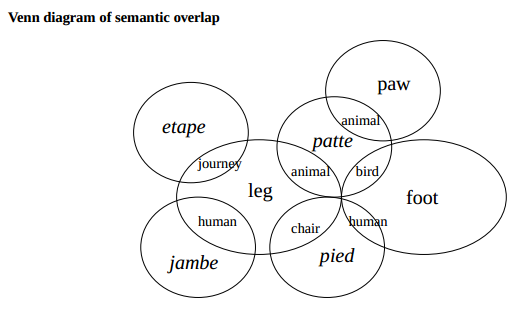
\includegraphics[width=12cm]{hutchins-leg-etc.png}
  \caption{Overlap of words related to ``leg"; relationships between English
  and French words. Figure 21.2 from \protect\cite{slp1}; example originally
  from \protect\cite[Chapter 6]{hutchins1992introduction}.}
  \label{fig:leg}
\end{figure}


